\ifdefined\included
\else
\documentclass[a4paper,11pt,twoside]{StyleThese}
\usepackage{amsmath,amssymb, amsthm}             % AMS Math
\usepackage[T1]{fontenc}
\usepackage[utf8x]{inputenc}
\usepackage{babel}
\usepackage{datetime}

\usepackage{silence}

\WarningFilter{minitoc(hints)}{W0023}
\WarningFilter{minitoc(hints)}{W0028}
\WarningFilter{minitoc(hints)}{W0030}

\usepackage{lmodern}
\usepackage{tabularx}
%\usepackage{tabular}
\usepackage{multirow}
\usepackage{xspace}

\usepackage{subfig}
\usepackage[inline]{enumitem}

\usepackage{hhline}
\usepackage[left=1.5in,right=1.3in,top=1.1in,bottom=1.1in,includefoot,includehead,headheight=13.6pt]{geometry}
\renewcommand{\baselinestretch}{1.05}

% Table of contents for each chapter

\usepackage[nottoc, notlof, notlot]{tocbibind}
\usepackage{minitoc}
\setcounter{minitocdepth}{2}
\mtcindent=15pt
% Use \minitoc where to put a table of contents

\usepackage{aecompl}

% Glossary / list of abbreviations

\usepackage[intoc]{nomencl}
\iftoggle{ThesisInEnglish}{%
\renewcommand{\nomname}{Glossary}
}{ %
\renewcommand{\nomname}{Liste des Abréviations}
}

\usepackage{etoolbox}
\renewcommand\nomgroup[1]{%
  \item[\bfseries
  \ifstrequal{#1}{A}{Number Sets}{%
  \ifstrequal{#1}{G}{Agents Beliefs and Action Models}{%
  \ifstrequal{#1}{N}{Navigation}{%
  \ifstrequal{#1}{O}{Ontology}{%
  \ifstrequal{#1}{R}{Referring Expression Generation}{%
  \ifstrequal{#1}{Z}{Controllable and Uncontrollable Agents Task Planning}{}}}}}}%
]}

\makenomenclature



% My pdf code

\usepackage{ifpdf}

\ifpdf
  \usepackage[pdftex]{graphicx}
  \DeclareGraphicsExtensions{.jpg}
  \usepackage[pagebackref,hyperindex=true]{hyperref}
  \usepackage{tikz}
  \usetikzlibrary{arrows,shapes,calc}
\else
  \usepackage{graphicx}
  \DeclareGraphicsExtensions{.ps,.eps}
  \usepackage[dvipdfm,pagebackref,hyperindex=true]{hyperref}
\fi

\graphicspath{{.}{images/}}

%% nicer backref links. NOTE: The flag ThesisInEnglish is used to define the
% language in the back references. Read more about it in These.tex

\iftoggle{ThesisInEnglish}{%
\renewcommand*{\backref}[1]{}
\renewcommand*{\backrefalt}[4]{%
\ifcase #1 %
(Not cited.)%
\or
(Cited in page~#2.)%
\else
(Cited in pages~#2.)%
\fi}
\renewcommand*{\backrefsep}{, }
\renewcommand*{\backreftwosep}{ and~}
\renewcommand*{\backreflastsep}{ and~}
}{%
\renewcommand*{\backref}[1]{}
\renewcommand*{\backrefalt}[4]{%
\ifcase #1 %
(Non cité.)%
\or
(Cité en page~#2.)%
\else
(Cité en pages~#2.)%
\fi}
\renewcommand*{\backrefsep}{, }
\renewcommand*{\backreftwosep}{ et~}
\renewcommand*{\backreflastsep}{ et~}
}

% Links in pdf
\usepackage{color}
\definecolor{linkcol}{rgb}{0,0,0.4} 
\definecolor{citecol}{rgb}{0.5,0,0} 
\definecolor{linkcol}{rgb}{0,0,0} 
\definecolor{citecol}{rgb}{0,0,0}
% Change this to change the informations included in the pdf file

\hypersetup
{
bookmarksopen=true,
pdftitle="Endowing the robot with the abilities to control and evaluate its contribution to a human-robot joint action",
pdfauthor="Amandine MAYIMA", %auteur du document
pdfsubject="Thèse", %sujet du document
%pdftoolbar=false, %barre d'outils non visible
pdfmenubar=true, %barre de menu visible
pdfhighlight=/O, %effet d'un clic sur un lien hypertexte
colorlinks=true, %couleurs sur les liens hypertextes
pdfpagemode=None, %aucun mode de page
pdfpagelayout=SinglePage, %ouverture en simple page
pdffitwindow=true, %pages ouvertes entierement dans toute la fenetre
linkcolor=linkcol, %couleur des liens hypertextes internes
citecolor=citecol, %couleur des liens pour les citations
urlcolor=linkcol %couleur des liens pour les url
}

% definitions.
% -------------------

\setcounter{secnumdepth}{3}
\setcounter{tocdepth}{2}

% Some useful commands and shortcut for maths:  partial derivative and stuff

\newcommand{\pd}[2]{\frac{\partial #1}{\partial #2}}
\def\abs{\operatorname{abs}}
\def\argmax{\operatornamewithlimits{arg\,max}}
\def\argmin{\operatornamewithlimits{arg\,min}}
\def\diag{\operatorname{Diag}}
\newcommand{\eqRef}[1]{(\ref{#1})}

\usepackage{rotating}                    % Sideways of figures & tables
%\usepackage{bibunits}
%\usepackage[sectionbib]{chapterbib}          % Cross-reference package (Natural BiB)
%\usepackage{natbib}                  % Put References at the end of each chapter
                                         % Do not put 'sectionbib' option here.
                                         % Sectionbib option in 'natbib' will do.
\usepackage{fancyhdr}                    % Fancy Header and Footer

% \usepackage{txfonts}                     % Public Times New Roman text & math font
  
%%% Fancy Header %%%%%%%%%%%%%%%%%%%%%%%%%%%%%%%%%%%%%%%%%%%%%%%%%%%%%%%%%%%%%%%%%%
% Fancy Header Style Options

\pagestyle{fancy}                       % Sets fancy header and footer
\fancyfoot{}                            % Delete current footer settings

%\renewcommand{\chaptermark}[1]{         % Lower Case Chapter marker style
%  \markboth{\chaptername\ \thechapter.\ #1}}{}} %

%\renewcommand{\sectionmark}[1]{         % Lower case Section marker style
%  \markright{\thesection.\ #1}}         %

\fancyhead[LE,RO]{\bfseries\thepage}    % Page number (boldface) in left on even
% pages and right on odd pages
\fancyhead[RE]{\bfseries\nouppercase{\leftmark}}      % Chapter in the right on even pages
\fancyhead[LO]{\bfseries\nouppercase{\rightmark}}     % Section in the left on odd pages

\let\headruleORIG\headrule
\renewcommand{\headrule}{\color{black} \headruleORIG}
\renewcommand{\headrulewidth}{1.0pt}
\usepackage{colortbl}
\arrayrulecolor{black}

\fancypagestyle{plain}{
  \fancyhead{}
  \fancyfoot{}
  \renewcommand{\headrulewidth}{0pt}
}

%\usepackage{MyAlgorithm}
%\usepackage[noend]{MyAlgorithmic}
\usepackage{algorithm}
\usepackage[noend]{algpseudocode}
\usepackage{comment}
\usepackage[ED=MITT-InfoTel, Ets=INSA]{tlsflyleaf}
%%% Clear Header %%%%%%%%%%%%%%%%%%%%%%%%%%%%%%%%%%%%%%%%%%%%%%%%%%%%%%%%%%%%%%%%%%
% Clear Header Style on the Last Empty Odd pages
\makeatletter

\def\cleardoublepage{\clearpage\if@twoside \ifodd\c@page\else%
  \hbox{}%
  \thispagestyle{empty}%              % Empty header styles
  \newpage%
  \if@twocolumn\hbox{}\newpage\fi\fi\fi}

\newcommand*{\algrule}[1][\algorithmicindent]{%
	\makebox[#1][l]{%
		\hspace*{.2em}% <------------- This is where the rule starts from
		\vrule height .75\baselineskip depth .25\baselineskip
	}
}

%%% to have lines in algorithm, from stackexchange
\newcount\ALG@printindent@tempcnta
\def\ALG@printindent{%
	\ifnum \theALG@nested>0% is there anything to print
	\ifx\ALG@text\ALG@x@notext% is this an end group without any text?
	% do nothing
	\else
	\unskip
	% draw a rule for each indent level
	\ALG@printindent@tempcnta=1
	\loop
	\algrule[\csname ALG@ind@\the\ALG@printindent@tempcnta\endcsname]%
	\advance \ALG@printindent@tempcnta 1
	\ifnum \ALG@printindent@tempcnta<\numexpr\theALG@nested+1\relax
	\repeat
	\fi
	\fi
}
% the following line injects our new indent handling code in place of the default spacing
\patchcmd{\ALG@doentity}{\noindent\hskip\ALG@tlm}{\ALG@printindent}{}{\errmessage{failed to patch}}
\patchcmd{\ALG@doentity}{\item[]\nointerlineskip}{}{}{} % no spurious vertical space
% end vertical rule patch for algorithmicx

\makeatother
 
%%%%%%%%%%%%%%%%%%%%%%%%%%%%%%%%%%%%%%%%%%%%%%%%%%%%%%%%%%%%%%%%%%%%%%%%%%%%%%% 
% Prints your review date and 'Draft Version' (From Josullvn, CS, CMU)
\newcommand{\reviewtimetoday}[2]{\special{!userdict begin
    /bop-hook{gsave 20 710 translate 45 rotate 0.8 setgray
      /Times-Roman findfont 12 scalefont setfont 0 0   moveto (#1) show
      0 -12 moveto (#2) show grestore}def end}}
% You can turn on or off this option.
% \reviewtimetoday{\today}{Draft Version}
%%%%%%%%%%%%%%%%%%%%%%%%%%%%%%%%%%%%%%%%%%%%%%%%%%%%%%%%%%%%%%%%%%%%%%%%%%%%%%% 

\newenvironment{maxime}[1]
{
\vspace*{0cm}
\hfill
\begin{minipage}{0.5\textwidth}%
%\rule[0.5ex]{\textwidth}{0.1mm}\\%
\hrulefill $\:$ {\bf #1}\\
%\vspace*{-0.25cm}
\it 
}%
{%

\hrulefill
\vspace*{0.5cm}%
\end{minipage}
}

\let\minitocORIG\minitoc
\renewcommand{\minitoc}{\minitocORIG \vspace{1.5em}}

\usepackage{multirow}
%\usepackage{slashbox}

\newenvironment{bulletList}%
{ \begin{list}%
	{\tiny$\bullet$}%
	{\setlength{\labelwidth}{25pt}%
	 \setlength{\leftmargin}{30pt}%
	 \setlength{\itemsep}{-0.5em}}}%
{ \end{list} }

\newenvironment{inlineEnumerate}
{\begin{enumerate*} [label={(\arabic*)}] }
{\end{enumerate*}}

\theoremstyle{definition}
\newtheorem{definition}{Definition}
\renewcommand{\epsilon}{\varepsilon}

% centered page environment

\newenvironment{vcenterpage}
{\newpage\vspace*{\fill}\thispagestyle{empty}\renewcommand{\headrulewidth}{0pt}}
{\vspace*{\fill}}

\newenvironment{asl}{\ttfamily\begin{tabbing}~~~\=$\leftarrow$ \= ~~~ \=
		\kill}{\end{tabbing}}

\usepackage{tablefootnote}

\theoremstyle{plain}
\newtheorem{constraint}{Constraint}[section]

\algnewcommand\algorithmicforeach{\textbf{for each}}
\algnewcommand\algorithmicin{\textbf{in}}
\algdef{S}[FOR]{ForEach}[2]{\algorithmicforeach\ #1\ \algorithmicin\ #2\ \algorithmicdo}

\algnewcommand\algorithmicforkxor{\textbf{do fork-join-xor}}
\algnewcommand\algorithmicendforkxor{\textbf{end fork-join-xor}}
\algdef{SE}{ForkXor}{EndForkXor}{\algorithmicforkxor}{\algorithmicendforkxor}


\usepackage{listings}
\lstset{
	frame=single,
	captionpos=b,
	breaklines=true,
	basicstyle=\ttfamily,
	numberstyle=\color{black},
	tabsize=2,
	mathescape=true,
	literate=%
		{â}{{\^a}}1
}

\lstdefinestyle{inline}{
	frame=none,
	aboveskip=\smallskipamount,
	belowskip=\smallskipamount,
}

\lstdefinestyle{OwlTurtle}{
	language=C,
	tabsize=4,
	basicstyle=\scriptsize\ttfamily,
	keywordstyle=\bfseries\color{darkgray},
	morekeywords={rdf:type, rdfs:domain, rdfs:subPropertyOf, rdfs:range, :hasSubtask, :DecompositionUsedBy, rdfs:subClassOf, :hasDecomposition, owl:inverseOf, htn_actions:hasEffect, rdfs:label},
	alsoletter=:
}

\lstdefinestyle{aslDef}{
	frame=none,
%	breaklines=false,
	%xleftmargin=.1\textwidth, xrightmargin=.1\textwidth
}

\fancypagestyle{example}{%
	\fancyhead[LE]{\bfseries\thepage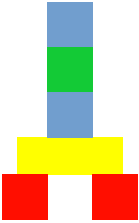
\includegraphics[scale=0.20]{figures/chapter2/task_goal.pdf}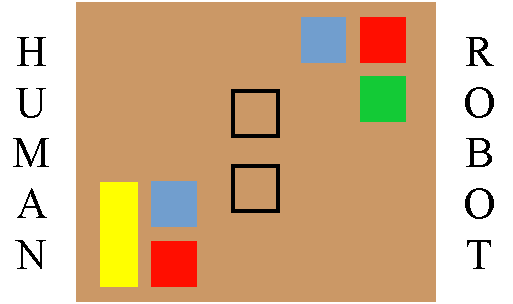
\includegraphics[scale=0.18]{figures/chapter2/task_setup_mini.pdf}}   
	\fancyhead[RO]{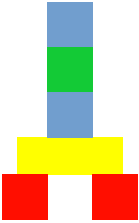
\includegraphics[scale=0.20]{figures/chapter2/task_goal.pdf}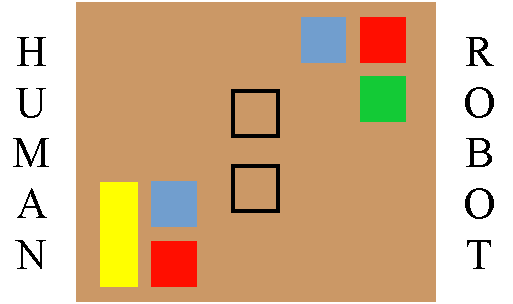
\includegraphics[scale=0.18]{figures/chapter2/task_setup_mini.pdf}\bfseries\thepage}  
	\fancyhead[RE]{\bfseries\nouppercase{\leftmark}}      % Chapter in the right on even pages
	\fancyhead[LO]{\bfseries\nouppercase{\rightmark}}     % Section in the left on odd pages
}%

\usepackage{pdfpages}
\usepackage{makecell}
\usepackage{pdflscape} 
\usepackage{mathtools}
\usepackage[section]{placeins}
\usepackage{afterpage}

%%%%%%%% my commands
\newcommand{\etal}{\textit{et al}.}
\newcommand{\ie}{\textit{i.e.}, }
\newcommand{\eg}{\textit{e.g.}, }
\newcommand{\fact}[3]{\mbox{\textit{#1}(#2, #3)}}
\newcommand{\circledtext}[1]{\raisebox{.5pt}{\textcircled{\raisebox{-.9pt} {#1}}}}
\newcommand{\sparql}{\textsc{SPARQL}}

\newcommand{\algConst}[1]{${\scriptscriptstyle #1}$}
\newcommand{\algNormTextSub}[2]{$\text{#1}_{#2}$}

\newcommand{\aslnumber}[1]{$#1$}
\newcommand{\aslstring}[1]{\textsf{#1}}
\newcommand{\aslvar}[1]{\textcolor{purple}{\textit{#1}}}
\newcommand{\asllabel}[1]{\textbf{#1}}
\newcommand{\annotation}[1]{{\footnotesize #1}}
\newcommand{\rulebody}[1]{\mbox{\hspace{.05\linewidth}}\begin{minipage}[t]{0.9\linewidth}#1.\end{minipage}}
\newcommand{\context}[1]{\begin{minipage}[t]{0.9\linewidth}#1\end{minipage}}
\newcommand{\planbody}[1]{\begin{minipage}[t]{0.9\linewidth}#1.\end{minipage}}
\newcommand{\Jason}[0]{\textbf{\textit{Jason}}}
\newcommand{\sn}{\mbox{\large\textbf{\texttt{\textasciitilde}}}}


\sloppy
\begin{document}
	\setcounter{chapter}{0} %% Numéro du chapitre précédent ;)
	\dominitoc
	\faketableofcontents
	\fi


\chapter{Lessons from Human-Human models}
\label{chapter:chap1}
\minitoc

When humans collaborate to achieve a task together, numerous neurocognitive mechanisms come into play, more than we would have thought at first glance. Some of these mechanisms are also triggered in humans’ minds when they interact with robots as they are essential to a successful collaboration. Therefore, it is important for roboticists designing robots that will closely interact with humans to be aware of and take into account the humans mental states and sensorimotor functions involved in controlling and smoothing collaborative task performance.  However, this does not imply that robots have to be endowed with the same mechanisms since being able to collaborate with humans does not mean to imitate them. What is key to roboticists is to understand how humans work and to design robots that will adapt. 

Consequently, this manuscript starts with an immersion in philosophy and social and cognitive psychology. We develop key elements for collaboration such as \acrlong{tom}, joint action and communication.

We focused on four main questions which were important to us, as roboticists, to design and develop our supervision software and integrate it in a robotic architecture dedicated to \acrshort{hri}. 

%\begin{samepage}
\begin{bulletList}
	\item What is a social interaction? (Section~\ref{chap1:sec:soc_int})
	\item How does one represent the others' mental states? (Section~\ref{chap1:sec:tom})
	\item What is a joint action? (Section~\ref{chap1:sec:ja})
	\item How does one person share information with another? (Section~\ref{chap1:sec:comm})
\end{bulletList}
%\end{samepage}

The answers to these questions, often captivating discussions, allowed us to extract structures and mechanisms of social interactions and collaboration. Thus, we were able to endow the robot with such elements, or at least we could draw our inspiration from. For example, we defined an \emph{interaction session} for collaborative robots (Chapter~\ref{chapter:chap5}) based on our readings on human-human social interactions (Section~\ref{chap1:sec:soc_int}). Or, the way the robot maintain knowledge about the shared plans with two different processes (Chapter~\ref{chapter:chap6}), one for itself and one for the robot, has been inspired by our study of the \acrlong{tom} (Section~\ref{chap1:sec:tom}).

\bigskip

Especially the reflection around the joint action concept and communication has been stimulated by the context of the JointAction4HRI project\footnote{https://jointaction4hri.laas.fr/}. This project gave us the opportunity to collaborate with Kathleen Belhassein, a PhD student in psychology, and V{\'\i}ctor Fern{\'a}ndez Castro, a post-doctoral researcher in philosophy. This collaboration led to three articles: a publication with a focus on communication, a publication under submission at Acta Psychologica~\cite{belhassein_2021_adressing} discussing joint action in \acrshort{hri} and a publication under submission in a volume of the Book Serie Techno:Phil~\cite{castro_2021_role} tackling commitments in \acrshort{hri}.

\section{What is a social interaction?}
\label{chap1:sec:soc_int}

\subsection{How to define a social interaction?}
First, let’s take a look at the dictionary and see how the word \emph{interaction} is defined. According to the Oxford dictionary, an interaction is a ``reciprocal action or influence'' and more precisely a ``communication or direct involvement with someone or something''. As for the Cambridge dictionary, it defines it as an occasion when two or more people or things communicate with or react to each other''. Those definitions can give a hint about what it an interaction between humans but they are not specific enough. 

Now, going through social psychology literature, one of the first attempts to define \emph{social interaction} was by Goffman~\cite{goffman_1967_interaction}. He distinguished three basic interaction units: the social occasion, the gathering and the social situation. The social occasion is an event that is temporally and spatially situated in such a way that it forms a unit that can be looked forward and back upon, by participants that are informed by the event (dinner, meeting, sport game...). The gathering refers to any set of two or more individuals who are at the moment in one another’s immediate presence. It can be noted that a social occasion may include several gatherings but that gathering do not need social occasions to occur (they can happen in office spaces, street corners, restaurants...). The social situation refers to the full spatial environment that embraces interacting people. It is created as soon as people engage in interaction, when mutual monitoring occurs and ends when the next to the last person leaves. Furthermore, Goffman distinguished between focused and unfocused interaction (gathering). A focused gathering has its members that can come together to sustain a joint focus of visual and cognitive attention and are open to each other for talk. He calls it encounters or engagements. On the other hand, an unfocused gathering has its members present to one another but not engaged together (\eg persons waiting for a bus). In this same book, Goffman proposed a definition of social encounter: ``an occasion of face-to-face interaction, beginning when individuals recognize that they have moved into one another’s immediate presence and ending by an appreciated withdrawal from mutual participation''.

A couple of years later, Argyle wrote a book entitled Social Interaction~\cite{argyle_1973_social}, where he laid the foundations to understand social interactions. He came to the view that social interaction could be interpreted as a set of social skills, and that it may therefore be possible to train these skills the same way as manual skills are trained. For example, during an encounter between two persons, each must be able to perceive the social cues (verbal or non-verbal signals) of the other which are then filtered through the perspective each has acquired through socialization and experience. The interpretation of context and social cues is then applied to come to a definition of the situation, which in turn guides both behavior and action.

Then, Rummel proposed a definition of a few words: ``Social interactions are the acts, actions, or practices of two or more people mutually oriented towards each other's selves, that is, any behavior that tries to affect or take account of each other's subjective experiences or intentions.''~\cite{rummel_1976_understanding}.

The elements brought here, trying to define what is an interaction and more precisely a social interaction. We chose the ones which were more relevant to us or the most referred to in the literature but large amount of work exists on this topic. So, it is possible to find different definitions than the ones we selected.

\subsection{Structure of a social interaction}\label{chap1:subsec:social_int}
Most of the research about social interaction belongs to the field of social psychology. As for the structure of a social interaction, it is more from the field of Conversation Analysis (CA) which mixes sociology, anthropology, linguistics, speech-communication and psychology.

Robinson makes a review of the work that has been done about \emph{overall structural organization}~\cite{robinson_overall_2012}. Most of the time in the literature, overall structural organization is discussed in terms of ``the overall structural organization of entire, single occasions of interaction''. Then, the \emph{overall structural organization} term is generally used to talk about one particular (albeit large) unit of interaction. However, many different types of interactional units can have an overall structural organization. For example, Schegloff encouraged to recognize ``‘overall structural organization’ not as something for the unit ‘a single conversation’ (or encounter, or session, etc.) alone, but for units like turns, actions and courses of action (like answering or telling), sequences, and who knows what else as well''~\cite{schegloff_2011_word}. He also mentioned that every unit of organization should probably have a local organization and a global organization. Here, the term \emph{overall structural organization} refers to ``the overall structural organization of entire, single occasions of interaction''. 

Robinson tells us that this concept has received relatively little analytic attention and thus is still not well understood~\cite{robinson_overall_2012}. Indeed, research has been more focused on analyzing the organization of individual sequences of action such as turn-takings or conversation openings. Several terms have been used to talk about a \emph{supra-sequential coherence}: big package, set of pre-organized sequences, (social) activity, project of activity or plan of action. Sacks gave the following definition for the overall structural organization of single occasions of interaction: it ``deals, roughly, with beginnings and endings, and how beginnings work to get from beginnings to something else, and how, from something else, endings are gotten to. And also the relationship - if there is one - between beginnings and endings''~\cite[p.~157]{sacks_lectures_1995}. Robinson summarized research about the subject by saying that single occasions of interaction (in a generic or context-free sense) are normatively organized as: (1) beginning with an opening (2) ending with a closing and (3) having ``something'' in between opening and closing'' which can be referred to as ``topics''~\cite{robinson_overall_2012}.

\subsubsection{Opening}
Openings are used to begin an encounter. One of the main reference on the subject is the work of Schegloff~\cite{schegloff_1986_routine}. Openings and related issues vary depending on the nature of interactions. For example, opening of a phone call to a family member or a friend will be organized as follow: (1) summons-answer (the one calling talks first) (2) identification/recognition of each other (3) greetings and (4) how-are-you. Whereas, in primary-care medical visits, opening is sequenced as: (1) greeting (2) securing patients’ identities (2) retrieving and reviewing patients’ records and (4) embodying readiness (sitting down and facing one another). More examples from the literature can be found in~\cite{robinson_overall_2012}. 

Another work, by Kendon~\cite{kendon_1990_conducting}, focuses on the greeting part, but more precisely the greeting behavior with the associated non-verbal cues. The greeting behavior is divided in three main phases: the distance salutation, the approach and the close salutation. 
The distance salutation only occurs if the greeters as far enough such as they need to get closer if they wish to continue the interaction. This phase starts after at least one participant sights the other and demonstrates a wish to engage in a greeting. In case one of the participant has not seen the other one, they signals their presence by vocalizing the other one’s name or by clearing their throat. Then, they orient their bodies towards each other and exchange glances in a subtle acknowledgement that the greeting is desired by both. During this phase, people can also wave or give a sign with their head (\eg nod).
The approach is divided into two sub-phases: the distant approach and the final approach. During the distant approach, people tend to look away whereas when the final approach starts (the greeters are 3 meters or less from one another), they look back at each other and, they smile.
Finally, there is the close salutation, the most normalized phase of the greeting. It happens when people are 1,5 meters or less from each others. Then, they can have a non-contact close salutation during which people exchange verbal greetings, or they can hand-shake or embrace (or do something else according to their culture). The greeting is over.

We should keep in mind that these studies and interaction analysis have been done in Western countries, and so that it is different in other cultures.

\subsubsection{Topics}
Episodes of social interaction, in a conversation context, vary a lot in their contextualized nature, which leads to a large variety of topics and sequences of topics. Interactions that happen in ordinary or institutional contexts can be pre-organized around one or more topics. Robinson gave examples such as an emergency call or an expected call back by a friend to discuss an expected single item of business~\cite{robinson_overall_2012}. 

\subsubsection{Closing}
Schegloff is one of the reference on closing as well~\cite{schegloff_1973_opening}. A closing can be divided into two phases: the topic termination and the leave-taking.
The topic termination has a pre-closing statement which signals to the partner the wish to close the conversation. Then, the leave-taking follows the pre-closing statement and its response and, includes the goodbye exchange. Finally, the partners break co-presence, \ie physically walk apart.\footnote{It is not explicitly mentioned in~\cite{schegloff_1973_opening}  but they precise in a footnote that it would not make sense if the parties remain in co-presence after having being through the closing sequence.} In the context of a phone call, Clark and French defined this co-presence breaking as the \emph{contact termination} when people hang up~\cite{clark_1981_telephone}.

With regards to non-verbal cues, Knapp \etal{} listed and analyzed them~\cite{knapp_1973_rhetoric}. The more frequent are eye contact breaking, head nodding, leaning toward the partner and positioning in the direction of the way of leaving.

\bigskip

Now that we have a pretty good idea of what is a social interaction, we are going to take an interest to how one represents what happens in another's mind during an interaction.

\section{How does one represent the others' mental states? -- Theory of Mind}~\label{chap1:sec:tom}
%\subsection{Theory of Mind}~\label{chap1:sec:tom}
\acrfull{tom} refers to the ability to represent others' intentions, beliefs, knowledge, goals, \ie their \emph{unobservable mental states}~\cite{premack_1978_does,povinelli_2004_we}. This concept is related to other ones which will be described in Section~\ref{chap1:sec:ja} such as common knowledge, shared intentions, joint attention and cooperation. Indeed, common knowledge requires \acrshort{tom} as ``to know what another knows and to be capable of making the sorts of inferences required for common knowledge, one must have an understanding of others (or an understanding of a particular person) in terms of thoughts and beliefs''~\cite[p.~82]{tollefsen_2005_let}. And thus, shared intention, as stated by Pacherie, ``having a shared intention typically presupposes cognitively and conceptually demanding theory of mind skills''~\cite[p.~1817]{pacherie_2013_intentional}. Moreover, some authors showed that \acrshort{tom} development and functioning relied on joint attention~\cite{sodian_2015_declarative, camaioni_2004_role}.  Finally, it has been shown that \acrshort{tom} improves joint planning and so increases the ability to cooperate in joint activity~\cite{astington_1995_theory}. We can note that Westby and Robinson explained that recent research about \acrshort{tom}, showed that \acrshort{tom} is not only to understand what others think, know, believe or intend (cognitive \acrshort{tom}) but that another part of \acrshort{tom} involves thinking about and experiencing the emotions of others (affective \acrshort{tom})~\cite{westby_2014_developmental}. In this thesis, we will leave aside the latter.

As for common knowledge (see Section~\ref{chap1:subsubsec:common_g}), there is an infinite number of levels, or orders to \acrshort{tom}. Most often, the focus is on the first and the second orders. Perner and Wimmer defined the ``first-order belief attribution'' as the estimation of one's beliefs (\eg I think she thinks that) and the ``second-order belief attribution'' as the estimation of what one  thinks about what another person is thinking or feeling (\eg I think she thinks I think that)~\cite{perner_1985_john}. Based on the same principle, Flavell \etal{} proposed levels of role-taking where the Level 1 is defined as ``S thinks (knows, predicts or whatever) that O has such-and-such belief (attitude, feeling, etc.) about something (X), about S himself, about O himself or about some other individual or group (O\textsubscript{1})'' (\eg ``I know how you feel (about something or someone)''). The level 2 is defined as ``S thinks that O is aware of (unaware of, dislikes, etc.) S's or O\textsubscript{1}'s thoughts (feelings, perceptions, etc.) regarding X, S, O or O\textsubscript{1}'' (\eg ``I'm sure you know what I think about Bill'')~\cite[pp.~49--51]{flavell_1968_development}.

\paragraph{And perceptive-taking} \acrshort{tom} is also closely related to another notion that we have not mentioned yet but that is of interest in \acrshort{hri}: perspective-taking, which is mostly studied in psychology, sociology and neurology. These fields study how people understand each others and refer to it in different ways: social perspective-taking or role-taking, perspective-taking or empathy~\cite{davis_2017_self,quesque_2020_theory}. Sometimes, \acrshort{tom} and perspective-taking are used interchangeably, as by Charlop-Christy and Daneshvar defining perspective-taking as an elementary aspect of \acrshort{tom}~\cite{charlop_2003_using} or \acrshort{tom} can be a synonym of ``cognitive perspective-taking''~\cite{barnes_2004_perspective}. 

While, some authors, like Westby and Robinson, differentiated them and showed that perspective-taking is an element among others of \acrshort{tom}~\cite{westby_2014_developmental}. Actually, the perspective-taking to which they referred is the one called \emph{visual perspective-taking} which is a type of \emph{perceptual perspective-taking}. Indeed, perspective-taking, as \acrshort{tom}, has several dimensions. Some authors distinguish between \emph{perceptual perspective-taking}, referring to the inference that a person makes regarding another person's visual, auditory, or other perceptual experience; and \emph{conceptual perspective-taking}, referring to the inference that one makes regarding another's internal experience such as their thoughts, desires, attitudes, plans~\cite{marvin_1976_early}. 

Others distinguish two different dimensions: ``\emph{cognitive perspective-taking} may be defined as the ability to infer the thoughts or beliefs of another agent, while \emph{affective perspective-taking} [or emotional~\cite{hynes_2006_differential}] may be defined as the ability to infer the emotions or feelings of another agent''~\cite{healey_2018_cognitive}. According to the task being performed, ``\acrlong{tom} could require emotional or cognitive perspective-taking, or both''~\cite[p.~375]{hynes_2006_differential}. Cognitive perspective-taking is central to communication, particularly in the creation and understanding of referring expression (\ie a word or phrase to identify an object)~\cite{krauss_1991_perspective}.

\bigskip

Another element of \acrshort{tom} that we will discuss is the ability to attribute false belief to others, \ie make the distinction between the reality and what one can believe about the world~\cite{dennett_1978_brainstorms}, as tasks demonstrating this ability have been extensively used to test theory of mind of individuals, such as the task created by Wimmer and Perner~\cite{wimmer_1983_beliefs} and then extended by Baron-Cohen \etal{} which is the most famous false belief task, the Sally--Anne test\footnote{It has been shown that false belief tasks are not enough to assess \acrshort{tom}~\cite{bloom_2000_two, wellman_2001_meta}.}~\cite{wimmer_1983_beliefs, baron_1985_does}. In the experiment, children are presented two characters, Sally (who has a basket) and Anne (who has a box). Then, Sally departs, leaving a object A in her basket. While Sally is away, Anne removes the object and hides it in her box. Children are asked to predict, on Sally's return to the room, where Sally will look for the object. Authors used to claim that children being able to answer to this question had \acrshort{tom} whereas others did not.

\bigskip

\acrlong{tom} can be considered as a facilitator of social interactions, included joint action which we will now present.

\section{What is a joint action?}\label{chap1:sec:ja}
Several models, concepts, exist to define the frame and the mechanisms into play during a collaborative tasks and some of them stand out from the crowd to help roboticists to develop collaborative robots: Joint Intentions by Cohen and Levesque~\cite{cohen_1991_teamwork}, Joint Activity by Klein \etal{}~\cite{klein_2005_common}, Shared Plans by Grosz and Klaus~\cite{grosz_1996_collaborative} or Joint Action by Sebanz \etal{}~\cite{sebanz_2006_joint}.

We chose to focus on joint action as the theoretical fundamentals for our work as there is a dynamic community of researchers, multidisciplinary studying the concept. For example, two workshops\footnote{https://fja.sciencesconf.org} are regularly held to discuss it since 2014: \textit{toward a Framework for Joint Action (FJA)} and \textit{Human-Robot Joint Action (HRJA)}. Moreover, we were involved in the JointAction4HRI project\footnote{https://jointaction4hri.laas.fr}.

Even though joint action is extensively studied, multiple concepts are interlaced with it and it not always clear how: collaboration, cooperation, coordination, joint action, joint activity, shared/joint attention, shared/joint intention, shared plan, shared/common/joint goal, (joint) commitment, engagement, mental states, theory of mind, mutual knowledge... Many terms and definitions, whether inside a field\footnote{Here, philosophy, psychology or robotics} or between fields do not reach a consensus. This can be quite confusing, especially for roboticists for which it is initially not the range of expertise. 

Thus, we will first give an overview of the more characteristic definitions of what is Joint Action. Then, we will present a non-exhaustive set of notions related to Joint Action, the ones we identified as interested for us, roboticists.

\subsection{How to define Joint Action?}\label{chap1:subsec:def_ja}

This section is the result of talks with Kathleen Belhassein and V{\'\i}ctor Fern{\'a}ndez Castro, study of the literature and analysis from a non-psychologist/philosopher point of view.

An important number of social interactions and encounters are encompassed by the notion of joint action. Broadly considered, joint action is any form of social interaction whereby two agents or more coordinate their actions in order to pursue a joint goal. However, the notion of joint action has particularly been subject to debate in philosophy and psychology. For instance, according to Sebanz \etal~\cite[p.~70]{sebanz_2006_joint}, ``joint action can be regarded as
any form of social interaction whereby two or more individuals coordinate their actions in space and time to bring about a change in the environment.''; while other authors~\cite{carpenter_2009_just, cohen_1991_teamwork, fiebich_2013_joint, tomasello_2005_understanding,pacherie_2012_agency} resist the idea that instances of mere coordination – \eg two partners walking side by side – constitute a joint action if they met some necessary conditions like sharing goals and intentions.

Moreover, while the notion of joint action is used interchangeably with the notion of \emph{collaboration} or \emph{cooperation} for some authors such as Becchio \etal~\cite{becchio_2010_toward} and Kobayashi \etal~\cite{kobayashi_2018_language}, other authors establish a hierarchy of interactions depending on the processes involved~\cite{amici_2015_coordination, chalmeau_1995_cooperation}. According to Amici and Bietti, for example, coordination is a fast low-level process of behavioral matching and interactional synchrony which could, but not necessarily, facilitate middle-level processes like cooperation, collaboration or high-level processes like joint action, which requires other resources like turn-taking and alignment of linguistic resources during dialogue. ``To date, however, little is known about the exact way in which coordination, collaboration and cooperation are linked to each other''~\cite[p.~vii]{amici_2015_coordination}. Looking at the APA dictionary, collaboration is ``the act or process of two or more people working together to obtain an outcome desired by all, as in collaborative care and collaborative learning'' and ``cooperation a process whereby two or more individuals work together toward the attainment of a mutual goal
or complementary goals. [...] Often cooperation leads to outcomes [...] but the benefit to each individual is not always obvious''~\cite{sharbrough_2015_apa}. Thus, here the nuance is in the process benefit and not in the temporal level.

If we look at Sebanz and colleagues definition of joint action, it could be considered as a kind of activity (based on the usual sense of the term activity). Thus, some authors use the concept \emph{joint activity} interchangeably with \emph{joint action}~\cite{tollefsen_2005_let,grafenhain_2013_three} while others see the joint activity composed of joint actions~\cite{clark_1996_using, feltovitch_2005_common}. Clark says that ``joint activities advance mostly through joint actions''~\cite[p~.59]{clark_1996_using}. He defines the properties of a joint activity among which there are: it is carried out by 2 or more participants, each participant has a public role or they try to establish and achieve joint goals, and they may have private goals. He also highlights the need for coordination: ``What makes an action a joint one, ultimately, is the coordination of individual actions by two or more people. There is coordination of both \emph{content}, what the participants intend to do, and \emph{processes}, the physical and mental systems they recruit in carrying out those intentions''~\cite[p~.59]{clark_1996_using}. 

Sometimes, it is also possible to come across \emph{collaborative activity}~\cite{tomasello_2005_understanding}, \emph{collaborative task}~\cite{brennan_2008_coordinating} or \emph{collaborative joint action}~\cite{godman_2013_we} (less frequent). Tomasello \etal{} claimed that ``collaborative activities require both an alignment of self with other in order to form the shared goal, and also a differentiation of self from other in order to understand and coordinate the differing but complementary roles in the joint intention''~\cite[p.~681]{tomasello_2005_understanding}. Carpenter, one of the author of this latter article, uses the terms \emph{collaborative activity} and \emph{joint activity} to refer to the same task but giving a social dimension to collaborative activity, being ``an end in itself rather than just a means of getting something done''~\cite[p.~384]{carpenter_2009_just}. For Pacherie, joint actions are performed by the partners in order to achieve the joint goal of a collaborative activity or joint activity~\cite{pacherie_2013_intentional}.

As we can see, it is not possible to propose a unified definition of these terms based on the literature. In this thesis, the word joint action will be used to indifferently refer to an activity/task composed of several (joint) actions, \ie a high level joint action or as a single action, but in both cases it will imply that it is a ``social interaction where two or more individuals coordinate their actions in pursuit of a common goal''~\cite{castro_2020_joint}. We will also use \textit{joint activity} to refer to high level joint actions. Moreover, \acrshort{hri} often refers to collaborative tasks when the robot and the human perform an activity together, thus, we will also use this term which we consider as involving joint actions.

\subsection{Two possible divisions around Joint Action}

Before going through the mechanisms involved in joint action, we will briefly present two divisions of joint action: a temporal division, \ie the different phases a joint action goes through, and a cognitive model for human agency \ie the different neurocognitive levels that are involved in joint action. It seemed necessary to present these two divisions as the processes related to joint action described in Section~\ref{chap1:subsec:necess_ja} are sometimes involved in one phase/level but not in another. 

\subsubsection{Temporal division of Joint Action}
As a joint action is a form of social interaction, it can also be divided in three phases as presented in Section~\ref{chap1:subsec:social_int}: an initiation, a body and a closing~\cite{heesen_2017_social}. Each phase has a role. First, the initial phase establishes among other things the joint commitment, \ie who is to participate, in what roles (these can vary during the interaction), what actions are there to be performed, and when and where they will be performed~\cite{clark_2006_social}. Then, in the body, participants coordinate to achieve their goal. Finally, ``to complete a joint action, participants first need to arrive at the mutual conviction that they are both indeed ready to terminate it''~\cite{heesen_2017_social}, if they achieved their goal for example.

At a lower level of joint action, when considering it as an action and not an entire social interaction, joint action can be seen as a process with two phases: planning and execution. Curioni \etal{} proposed a model, specifying what happens in each phase~\cite{curioni_2017_joint}: 
\begin{bulletList}
	\item planning: 
	\begin{bulletList}
		\item expectations on partner's intentionality
		\item selecting action possibilities
		\item establishing commitment
	\end{bulletList}
	\item execution:
	\begin{bulletList}
		\item aligning attention to objects and events
		\item maintaining commitment
	\end{bulletList}
\end{bulletList}
\subsubsection{Neurocognitive division of Joint Action}~\label{chap1:subsubsec:neuro_seg}

To describe the levels of the neurocognitive mechanisms involved in joint action, we will base ourselves on the conceptual framework of action established by Pacherie~\cite{pacherie_2008_phenomenology}. This framework is particularly relevant for the rest of thesis as it has a lot similarities with the three-layered robotic architecture that will be described in Section~\ref{chap3:sec:rob_archi}, as discussed in~\cite{clodic_2017_key}. It is based on a dynamic model of intentions and distinguishes:

\begin{bulletList}
	\item A distal intentions level (D-intentions) in charge of the dynamics of decision making, temporal flexibility and high level rational guidance and monitoring of action;
	\item A proximal intentions level (P-intentions) that inherits a plan from the previous level and whose role is to anchor this plan in the situation of action, this anchoring has to be performed at two levels: temporal anchoring and situational anchoring;
	\item A motor intentions level (M-intentions) -- which encodes the fine-grained details of the action (corresponding to what neuroscientists call motor representations) -- is responsible for the precision and smoothness of action execution, and operates at a finer time scale than either D-intentions or P-intentions
\end{bulletList}

This model of action has then been enriched with the specificities of joint action in~\cite{pacherie_2012_agency}, integrating at each levels the representations and processes associated to the joint` action partner. We will not go through the details of it here but they will be mentioned all along the next section.

\subsection{What is necessary for Joint Action?}\label{chap1:subsec:necess_ja}

This section is the result of talks with Kathleen Belhassein and V{\'\i}ctor Fern{\'a}ndez Castro, study of the literature and analysis from a non-psychologist/philosopher point of view.

Leaving aside the debate on the concept of joint action, we aim to focus on the mechanisms that enable the consecution of joint actions. What we found to be the mechanism on which every author (or almost) agrees on to say that it is required for a joint action is the \emph{coordination}. This mechanism itself is supported by other cognitive and sensorimotor processes. Also, philosophers introduced another concept involved in joint action which is the \emph{shared intention}. 

When thinking about a way to organize this section, studying how the multiple mechanisms around joint action were linked together, we found that it was complicated as some of them intertwined. Thus, after a thorough analysis, we devised Figure~\ref{chap1:fig:ja}. It is an attempt to represent a number of these processes (the ones one which we focused and that were important for us as roboticists) and how they are connected to each other. It should be seen as a guide and an interpretation of the literature.

\begin{figure}[!htb]
	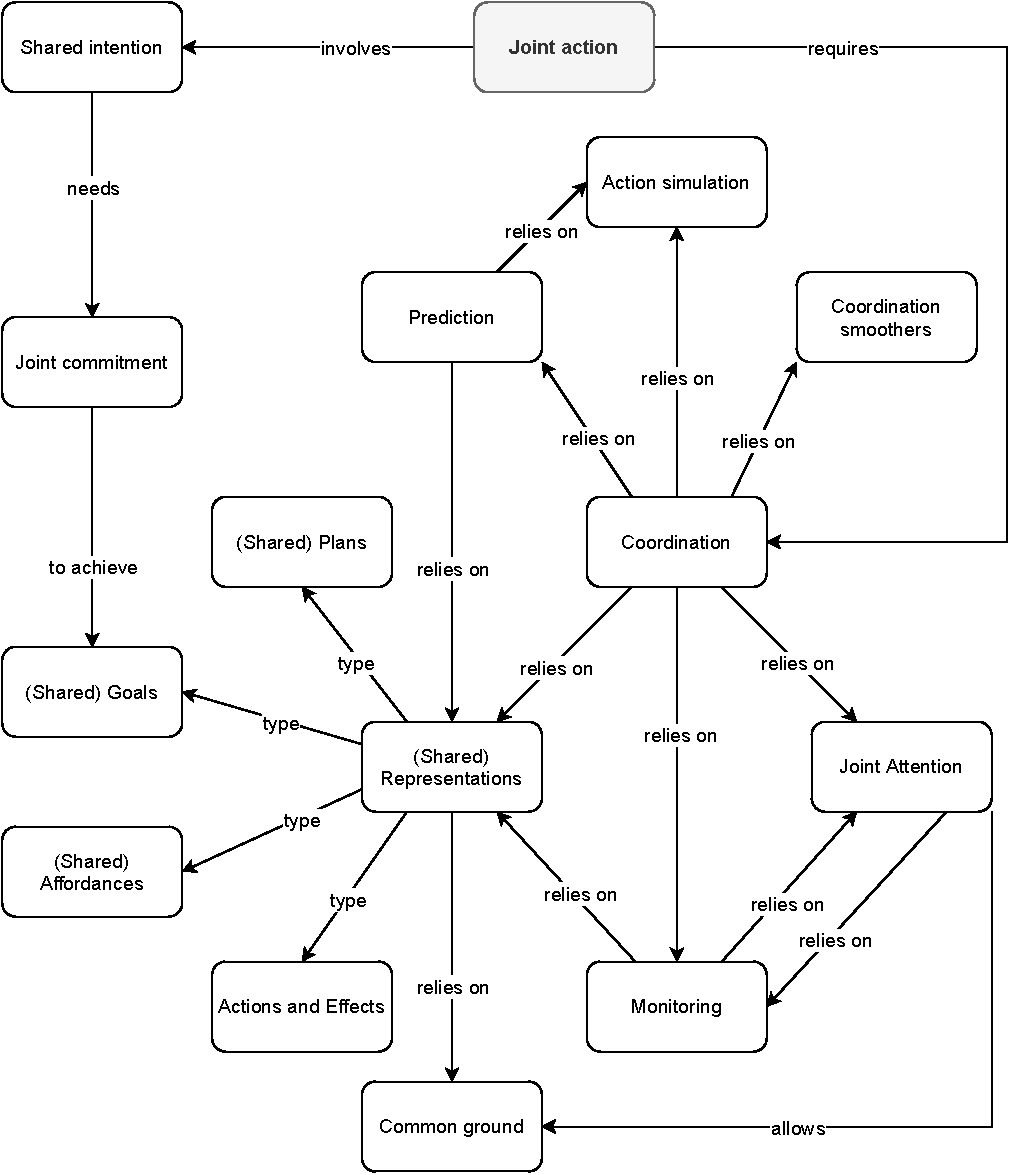
\includegraphics[width=\linewidth]{figures/chapter1/joint_action.pdf}
	\caption{Mapping of the processes we focused on related to joint action.}
	\label{chap1:fig:ja}
\end{figure}

We will first present the concepts of \emph{shared intention} and \emph{joint commitment} and then define the concept of \emph{coordination} and its associated mechanisms. 

\subsubsection{Shared Intention}
First, before coming to the concept of shared intention, what is an intention? We are going to take a look at three definitions, first from a philosopher (Bratman), then from computer scientists (Cohen and Levesque) and finally from psychologists (Tomasello \etal). 

Sometimes, we talk about intention to refer to something we do intentionally (action) or to refer to things we intend to do (mental state). Thus, Bratman distinguishes both~\cite{bratman_1984_two} associating the first possibility to what he calls ``present-directed intention'' (I may intend to start my car now) and the latter to ``future-directed intention'' (I may intend to start my car later today). But, ``when I am starting my car it may seem natural to say that I no longer intend to start it, I am starting it''~\cite[p.~379]{bratman_1984_two}. He chose to concentrate on future-directed intentions rather than present-directed intentions when referring to intentions. 

Cohen and Levesque based their definition of intention on this view of Bratman~\cite{cohen_1990_intention}. They added the notions of commitment and goal: ``An intention is defined as a commitment to act in a certain mental state: An agent intends relative to some conditions to do an action just in case she has a persistent goal (relative to that condition) of having done the action, and, moreover, having done it, believing throughout that she is doing it''~\cite[p.~496]{cohen_1991_teamwork}. 

The definition of Tomasello \etal{} includes the notion of plan since they defined an intention as ``a plan of action the organism chooses and commits itself to in pursuit of a \emph{goal}. An intention thus includes both a means (action \emph{plan}) as well as a goal'' (not yey executed)~\cite[p.~676]{tomasello_2005_understanding}. 

Now that we have a clearer idea of an intention, we can focus on shared intention. We will start again with Bratman~\cite{bratman_1993_shared}. He considers that two agents have the shared intention to J if and only if they think: 
\begin{enumerate}
	\item (a) I intend that we J and (b) you intend that we J.
	\item\relax I intend that we J in accordance with and because of 1a, 1b, and meshing subplans of 1a and 1b; you intend that we J in accordance with and because of 1a, 1b, and meshing subplans of 1a and 1b.
	\item 1 and 2 are \emph{common knowledge} between us.
\end{enumerate}

Tomasello, \etal{}, them, use the terms shared intentionality (``we'' intentionality) and joint intention~\cite{tomasello_2005_understanding}. For them, ``shared intentionality [...] refers to collaborative interactions in which participants have a \emph{shared goal} (\emph{shared commitment}) and coordinated action roles for pursuing that shared goal''. They based this definition on the work of Gilbert~\cite{gilbert_1989_social}, Searle~\cite{searle_1983_intentionality} and Tuomela~\cite{tuomela_1995_importance}. They defined joint intention as a form of shared intentionality where each partner's ``representation of the intention [...] contains both self and other'', as we can see in their illustration, reproduced in Figure~\ref{chap1:fig:ji}. We can also find other close terms such as Bratman who referred to Searle and Tuomela about their definition of ``we-intention'', highlighting the difference with shared intention. He explained that ``we-intentions'', also called ``collective intentions'' are intention of an individual concerning a group's or collective's activity, and there can be such intention even though there is only one individual (falsely believing others are involved)~\cite{bratman_1993_shared}. Whereas, a shared intention necessarily involved at least two persons. Thus, it can be compared with Tomasello \etal{}'s definition of joint intention. Some authors such as Tollefsen use joint intention and shared intention interchangeably~\cite{tollefsen_2005_let}.

 \begin{figure}[!ht]
 	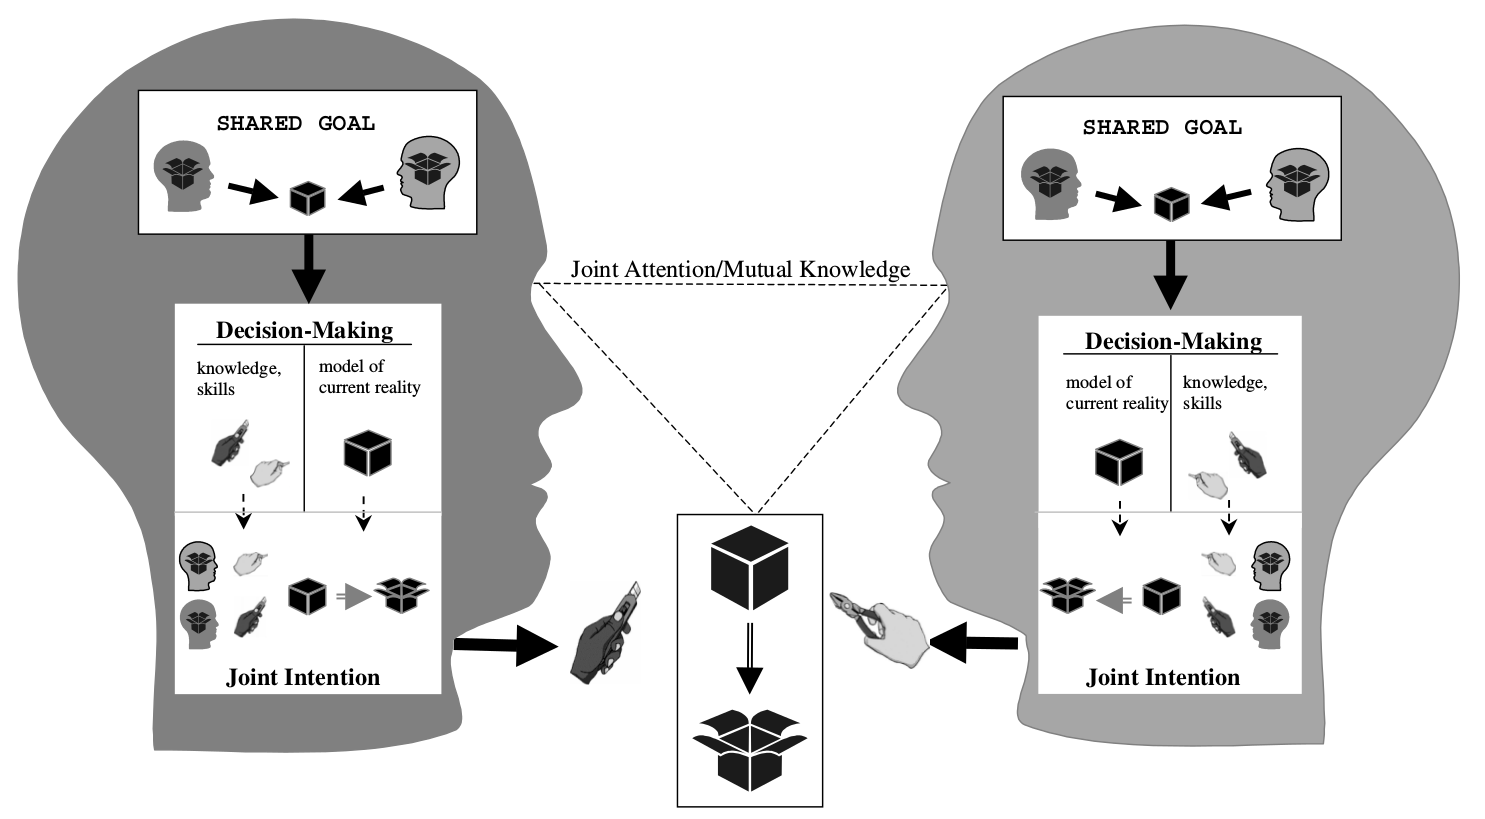
\includegraphics[width=\linewidth]{figures/chapter1/shared_representation.png}
 	\caption{Illustrative example of a collaborative activity by Tomasello \etal~\cite{tomasello_2005_understanding}. Here the humans have for shared goal to open the box together. They choose a means to perform it which takes into account the other's capabilities and so form a joint	intention.}
 	\label{chap1:fig:ji}
 \end{figure}

Cohen and Levesque took their inspiration from Bratman's definition of shared intention in their view of joint intention for artificial agents, considering joint intention as a future-directed \emph{joint commitment} to perform a collective action while in a joint (or shared) mental state.

\subsubsection{Joint Commitment}\label{chap1:subsubsec:joint_commit}
This section is composed of excerpts from the publication under submission in a volume of the Book Serie Techno:Phil~\cite{castro_2021_role}.

Commitments can be understood as ``a triadic relation among two agents and an action, where one of the agents is obligated to perform the action as a result of having given an assurance to the other agent that she would do so, and of the other agent’s having acknowledged that assurance under conditions of common knowledge''~\cite[p.~756]{michael_2017_commitment}. Commitments are not necessarily established through promises or even explicit verbal communication~\cite{ledyard_1994_public, scanlon_2000_we, siposova_2018_communicative}, however, this basic definition allows us to see the fundamental component of a commitment. But why are commitments important for joint action?

Many authors, in philosophy and psychology, have emphasized the importance of commitments for joint action such as Cohen and Levesque~\cite{cohen_1991_teamwork}, Clark~\cite{clark_2006_social}, Gilbert~\cite{gilbert_2009_shared}, Bratman~\cite{bratman_2014_shared}, Michael and Pacherie~\cite{michael_2015_commitments}, Roth~\cite{roth_2014_shared} or Siposova \etal~\cite{siposova_2018_communicative}. 

For instance, in philosophy, Gilbert~\cite{gilbert_2009_shared} and Bratman~\cite{bratman_2014_shared} have largely argued about the requirements for people to establish shared intentions and their role in explaining social coordination. While Bratman has argued that shared intentions can be understood as an aggregation of individual intentions which only requires individual commitments with general standards of rationality, Gilbert has argued that shared intentions are essentially tied to joint commitments. According to her, two or more persons share an intention to do something if and only if they are jointly committed to intend as a body to do it~\cite{gilbert_2009_shared}. In other words, joint actions require the people involved to impose obligations to each other. Further, Roth has argued that joint action requires the participants to be committed to the activity in the Gilbert’s sense, which also implies contralateral commitments that hold across the other participants in the shared activity~\cite{roth_2014_shared}. For instance, if Sue and Jack agree on going for a walk together, they share a commitment to carry out the shared action but also, they assume an individual contralateral commitment to keep pace with each other. In brief, commitments are essential for the establishment of joint and individual intentions during shared activities. 

In psychology, several authors, such as Clark~\cite{clark_2006_social}, Michael \etal~\cite{michael2016} or Siposova \etal~\cite{siposova_2018_communicative}, have studied how implicit and explicit communication are used to establish commitments and their importance for coordinated actions. For example, Clark has emphasized how partners use communicative exchanges like ``projective pairs'', where one of the participants proposes a particular goal to another (Let’s do G! Should we do that?), who then accepts or rejects the proposal~\cite{clark_2006_social}. Those exchanges are pervasive in human-human coordinated actions and they serve to negotiate goals, plans and social roles which are translated into an amalgamate of different types of commitments that are necessary for the execution of the general \emph{joint goal}. Michael \etal{} suggest that people often use investment of effort in a task as an implicit cue for making the perceiver aware that we expect him to behave collaboratively which often triggers a sense of commitment that motivates actions~\cite{michael2016}. Furthermore, Siposova \etal{} have found that humans use implicit cues like gaze signals to communicate an agreement or commitment to carry out a task their partner intends to perform~\cite{siposova_2018_communicative}.

The most important about joint commitment can be summarized with the words of Gilbert~\cite[p.~7]{gilbert_2013_joint}: ``a joint commitment is a commitment of the two or more people involved. It is, more fully, a commitment by two or more people of the same two or more people'', keeping in mind that it ``is not a concatenation of personal commitments''. 

\subsubsection{Coordination}
Coordination is a central mechanism to distinguish individual actions from joint actions. There has been an important deal of conceptual and empirical work investigating this process, such as the one of Knoblich \etal~\cite{knoblich_2011_joint} and the one of Pacherie~\cite{pacherie_2012_agency}. Coordination relies on several mechanisms (see Figure~\ref{chap1:fig:ja}). They can be non-intentional -- sometimes called emergent coordination~\cite{knoblich_2011_joint} -- such as perception-action matching~\cite{brass_2001_movement}, perception of joint affordances~\cite{ramenzoni_2008_short} or action simulation~\cite{sebanz_2009_prediction}. As for intentional coordination – sometimes referred to as planned coordination~\cite{knoblich_2011_joint} –, it requires the partners: (i) to represent their own and others' actions, as well as the consequences of these actions, (ii) to represent the hierarchy of sub-goals and sub-tasks of the plan, (iii) to generate predictions of their joint actions, and (iv) to monitor the progress toward the joint goal in order to possibly compensate or help others to achieve their contributions~\cite{pacherie_2012_agency}. 

From Section~\ref{chap1:subsubsec:shared_rep} to Section~\ref{chap1:subsubsec:coord_smooth}, we present a number of joint action mechanisms on which coordination relies. We chose the ones that seemed: to be the most mentioned in the philosophy and psychology literatures, to obtain consensus about their involvement in coordination and to be relevant to Human-Robot Interaction. 

\subsubsection{(Shared) Representations}\label{chap1:subsubsec:shared_rep}
As stated by Sebanz \etal, joint action depends on the ability to share representations~\cite{sebanz_2006_joint}. Representation sharing is present at different levels, \ie agents can share representations of objects, events, actions, goals, plans and tasks~\cite{pacherie_2012_agency,vesper_2017_joint}. These representations enable, among other things, the prediction (see Section~\ref{chap1:subsubsec:pred}) of other's actions. 

\paragraph{Representation of (Shared) Tasks}
A task can be described at multiple grains or levels of abstraction~\cite{cooper_2000_contention},  the same action can be described
as both ‘putting a piece of toast in one’s mouth’ and ‘maintaining an adequate supply of nutrients’. A used definition in psychology is that ``a task consists of producing an appropriate action (\eg conveying to mouth) in response to a stimulus (\eg toast in a particular context)''~\cite[p.~1]{monsell_2003_task}. Sebanz \etal{} extended this definition with the possibility to execute more than one action when responding to a stimulus~\cite{sebanz_2005_two}. 

How to share a task? Sebanz \etal{} proposed that ``sharing a task representation or corepresenting a task then means that an individual represents at least one rule that states the stimulus conditions under which a coactor should perform a certain action''~\cite[p.~1235]{sebanz_2005_two}.
In another paper, in the context of joint action, Sebanz \etal{} evoked studies showing the formation of shared representations during collaborative tasks, \ie an agent knows what the other should do and represents it in a functionally equivalent way to their's own. They concluded that it allowed individuals ``to extend the temporal horizon of their action planning,
acting in anticipation of others’ actions rather than simply responding''~\cite[p.~73]{sebanz_2006_joint}.


\paragraph{Representation of (Shared) Goals}
Goal has two meanings leading sometimes to ambiguities: the state-to-reach of the environment (external goal) and the mental representation of a desired state (internal goal)~\cite{tomasello_2005_understanding}. It is interesting to be aware of this double meaning. 

Several authors highlighted the need of the representation of a shared goal for joint action such as Pacherie~\cite{pacherie_2012_agency}, Tomasello \etal{}~\cite{tomasello_2005_understanding} or Cohen and Levesque~\cite{cohen_1991_teamwork}. Sometimes they use the terms  common goal~\cite{searle_1990_collective}, joint goal or joint persistent goal.
Based on Braman~\cite{bratman_1992_coop}, Tomasello \etal{} affirmed that ``there is a shared goal in the sense that each participant has the goal that we (in mutual knowledge) do X together'' and that ``each interactant has goals with respect to the other’s goals''~\cite{tomasello_2005_understanding}. Pacherie listed as a condition for joint action that each agent has to represent their goals and their coagents goals~\cite{pacherie_2012_agency}.

\paragraph{Representation of (Shared) Plans}
An intention is sometimes defined as a plan of actions that an agent chooses to achieve a given goal~\cite{tomasello_2005_understanding, kaplan_2006_challenges}. 
As for shared goals, Tomasello \etal{} and Pacherie highlighted the need for an agent to represent ``their own subplans and the meshing parts of the subplans of others, and some of what they represent is to be performed by others''~\cite[p.~353]{pacherie_2012_agency}.

Representations, models of plans and shared plans are more studied by computer scientists than by philosophers and psychologists, proposing computational models such as the ones of Grosz and Kraus. They demonstrated that shared (collaborative) plans should not be treated as the sum of individual plans but as plans necessitating from the agents joint intentions, a mutual belief of how to perform the task and eventually individual or shared plans to perform the task's actions~\cite{grosz_1996_collaborative}.

\paragraph{Representation of Actions and Effects}
Studies showed that when an agent observes an action, a corresponding representation in their action system is activated~\cite{rizzolatti_2004_mirror}. Sebanz \etal{} affirmed that representation sharing is essential to joint action, specially action representations, as ``individuals could be ‘on the same page’ action-wise by sharing representations of actions and their underlying goals''~\cite[p.~71]{sebanz_2006_joint}. Pacherie evokes the need of agents to have the ability to have not only a representation of actions to be performed, self's and other's, but also their consequences~\cite{pacherie_2012_agency}. 

\paragraph{Affordances}
The concept of affordances has been introduced in 1966~\footnote{\url{https://www.merriam-webster.com/dictionary/affordance}} by Gibson, a psychologist, who presented his theory of affordances in~\cite{gibson_1979_theory}. He coined the term to refer to what the environment has to offer to the animal (individual), ``what it provides or furnishes, either for good or ill''. Then, the term and concept became popular and have been used in other fields than the original one (ecological psychology) such as cognitive psychology, human-computer interaction or design. Osborne discussed in his thesis~\cite{osborne_2014_ecological}, among other things, the history of the word and the different uses and meaning there are nowadays (see also two reviews on affordances~\cite{jamone_2016_affordances, bach_2014_affordance}). The definition that is commonly used in HCI/HRI has been introduced by Norman, a design researcher, in 1988 which claimed that ``affordance refers to the perceived and actual properties of the thing, primarily those fundamental properties that determine just how the thing could possibly be used''~\cite[p.~9]{norman_1988_psychology}. Thus, it became associated to the term \emph{action possibilities}. 

What about affordances when people are in a joint action? Richardson \etal{} showed that when acting together, people take into account not only their motor affordances but also the ones of their partners, helping to decide whether to perform a joint action or an individual action with an object~\cite{richardson_2007_judging}. Thus, Knoblich \etal{} called \emph{common affordance} ``when two agents have similar action repertoires and perceive the same object [will likely] engage in similar actions because the object affords the same action for both of them''~\cite[p.~63]{knoblich_2011_joint}, enabling coordination as agents perceive the same objects at the same time. They called \emph{joint affordance} when ``objects have an affordance for two or more people collectively [(a two-handled saw)] which is not necessarily an affordance for any of them individually''.


\subsubsection{Joint Attention}\label{chap1:subsubsec:joint_att}
We will start with two complementary definitions of \emph{attention}. The first one is from Tomasello \etal{} who say ``attention may thus be thought of as intentional perception (selective attention)''~\cite{tomasello_2005_understanding}. The second one is from Kaplan and Hafner~\cite{kaplan_2006_challenges} who define attention as ``the temporally-extended process whereby an agent concentrates on some features of the environment to the (relative) exclusion of others''. They distinguish two situations for which the process can occur: (1) passive attention when a salient event happens and thus automatically triggers the attention of the agent, and (2) active attention when the agent is involved in an
intentionally directed process and must actively select particular features of its environment. 

What happens to this process in the context of a joint action? We then talk about \emph{joint attention}. To perform a joint action, partners need a common goal. Indeed, joint action requires that individuals plan and perform their actions according to their predictions about the other’s actions to reach this goal. Joint attention is a key feature for this purpose, playing a crucial role in ``being and acting together''~\cite{tomasello_2009_cultural}, as it allows the partners to establish and share a perceptual common ground, necessary to initiate the joint action but also for individuals already engaged in a joint action to coordinate successfully. 

Despite this agreement to affirm that joint attention is important for joint action, Siposova stated that ``there is still surprisingly little agreement on exactly what joint attention is and how it is achieved''~\cite{siposova_2019_new}. While for some authors, two agents orienting their attention towards the same referent is a sufficient criterion to speak about joint attention~\cite{butterworth_1991_minds}, others like Pacherie precised that ``the phenomenon of joint attention involves more than just two people attending to the same object or event''. A classic way to define joint attention is the ability to coordinate our attention to the same object of interest (\eg as shown by Bakeman and Adamson~\cite{bakeman_1984_coordinating}), enabling us to integrate others’ attentional focus and therefore to experience the world together as described by Tomasello~\cite{tomasello_2009_cultural}.  ``The attentional focus of the two persons must be truly joint in the sense that both participants are \emph{monitoring} the other's attention to the outside entity''~\cite[p.~106]{tomasello_1995_joint}, thus joint attention cannot exist without mutual knowledge (see Section~\ref{chap1:subsubsec:common_g}).

To complete this view of joint attention, we can mention Carpenter and Liebal that highlighted the need (1) to develop mutual knowledge of this coordinated attention, and (2) to represent the other agent’s intentional states~\cite{carpenter_2011_joint} or Kaplan and Hafner that make the notion of \emph{goal} appear in their definition, describing joint attention as (1) a coordinated and collaborative coupling between intentional agents where (2) the goal of each agent is to attend to the same aspect of the environment~\cite{kaplan_2006_challenges}.

%Joint attention can either be explained with basic learning mechanisms -- lean joint attention -- or as ``the result of particular cognitive operations or second-order representational competencies''~\cite{racine_2011_getting}, \ie what Tomasello and Carpenter called socio-cognitive abilities of shared intentionality~\cite{tomasello_2007_shared} -- rich joint attention. 
Kaplan and Hafner noticed in 2006 that current research in HRI about joint attention tended to focus on ``surface behaviors'', like simultaneous looking or coordinated behaviors~\cite{kaplan_2006_challenges} and not what Tomasello and Carpenter called socio-cognitive abilities of shared intentionality~\cite{tomasello_2007_shared}.
% which corresponds to lean joint attention.\todo{check si evolution depuis 2006}

Finally, sometimes it is possible to see references to \emph{shared attention} in the literature, which can be confusing for the reader when no precision or definition is given, differentiating it from \emph{joint attention} or not. Some authors use the two words interchangeably, while some consider that there is a difference between both. There are especially two work mentioning this fact and making a distinction, the one of Emery~\cite{emery_2000_eyes} and a bit later the one of Triesch \etal~\cite{triesch_2006_gaze}. They define joint attention as two people having the same focus of attention while they define shared attention as a more complex form of communication where each agent knows on what the other agent is focused. We can notice that it is quite similar to the definitions of joint attention we gave above.

\subsubsection{Common Ground}\label{chap1:subsubsec:common_g}
Common ground, or common knowledge or mutual knowledge, or mutual belief, these are the words to refer to the same general idea -- used by some authors interchangeably~\cite{clark_1992_arenas, clark_1996_using} -- but sometimes with nuances like for joint attention. Lewis, a philosopher, claims that a proposition P is commonly known among two agents if the proposition is known by the two agents and both agents know that agent A can draw the same conclusions from P that agent B can and vice-versa.~\cite{lewis_1969_convention}. In another famous formulation of philosophers~\cite{schiffer_1972_meaning} and psychologists~\cite{thomas_2014_psychology}, common knowledge must be understood as the recursive belief in which S knows P, Y knows P, S knows that Y knows P, Y knows that S knows P, S knows that Y knows that S knows P, and so on. The subject does not necessarily represent the whole line of reasoning beforehand but should be able to infer it. Thus, we can assume that from the individual point of view, common knowledge or common ground is the information that one may reasonably assume that one and her partner know and they can also know or infer that the other knows. For our purpose, such information may include goals and sub-goals, intentions (see~\cite{bratman_1992_coop}), ways to proceed, facts on the environment (see joint attention in Section~\ref{chap1:subsubsec:joint_att}), appropriate scripts and roles, and any other type of information necessary or relevant for the joint action. Cohen and Levesque, computer scientists, consider mutual knowledge about a \emph{joint persistent goal} P, such as ``it is true (and mutual knowledge) that until they come to mutually believe that P is true, that P will never be true, or that [the condition] Q is false, they will continue to mutually believe that they each have P as a weak achievement goal relative to Q and with respect to the team''~\cite[p.~499]{cohen_1991_teamwork}.

\subsubsection{Monitoring}\label{chap1:subsubsec:monitoring}
An agent can monitor multiple things related to a task: a goal, an action, a task-progress, mistakes, another agent, an object... Vesper \etal{} showed that an agent typically monitors the task-progress in order to determine whether the current state of the joint action and the desired outcome are aligned~\cite{vesper_2010_minimal}. Pacherie named the monitoring of the progress towards the joint goal as a condition for agent to share a proximal intention~\cite{pacherie_2012_agency}. Monitoring the task-progress is not enough. An agent also needs to monitor its partner, especially through joint attention that we presented in Section~\ref{chap1:subsubsec:joint_att}, as attention is a monitoring process and joint attention can be seen as the co-actors’ ability to monitor each other’s gaze and attentional states~\cite{emery_2000_eyes}. Then, it is also closely related to the shared representations we presented in Section~\ref{chap1:subsubsec:shared_rep}. Indeed, shared task representations enables the monitoring of the individual actions~\cite{knoblich_2011_joint}. Sebanz \etal{} mentioned ``action observation'' which seems to be an equivalent to the term monitoring\footnote{https://www.merriam-webster.com/thesaurus/monitoring}. Action observation and thus monitoring is based on action representations and allows to predict (see Section~\ref{chap1:subsubsec:pred}) what others are going to do next~\cite{sebanz_2006_joint}. Finally, ``monitoring is useful to detect mistakes or unexpected outcomes in one's own or one's partner's performance, enabling one to quickly react and adapt accordingly''.

\subsubsection{Action Simulation}
Sebanz \etal{} highlighted the need of action simulation for agents to coordinate~\cite{sebanz_2009_prediction,knoblich_2011_joint}. Action simulation is the process allowing an agent to predict the timing and outcomes of the given action, by observing the action and applying predictive models of the action in their motor system. Thus, an agent can predict other agents' actions in real time~\cite{wolpert_2003_unifying}.

\subsubsection{Predictions}\label{chap1:subsubsec:pred}
For Pacherie, there are three types of predictions: self-predictions, other-predictions, joint predictions. Self-predictions are the predicted consequences of the agent's own actions. Other-predictions concern predictions regarding the actions, goals, motor and proximal intentions of their coagent and their consequences. Joint predictions are the agents' prediction of the joint effects of their own and others' actions. These predictions allow agents to ``decide on their next moves, including moves that may involve helping others achieve their contributions to the joint goal (triadic adjustment)''~\cite[pp.~354-355]{pacherie_2012_agency}. Sebanz \etal{} support the same idea, claiming that predictions, based either on action observation or on shared representations, ``allow one to prepare actions in responses to events''~\cite[p.~73]{sebanz_2006_joint}.

\subsubsection{Coordination Smoothers}~\label{chap1:subsubsec:coord_smooth}
Coordination smoothers, as their name implies, are one way to facilitate coordination. They are defined as the changes in an agent own behavior to ease the interaction with another one~\cite{vesper_2010_minimal}. For example, an agent may exaggerate their movements, making them easier to predict for their partner. The change of behavior may concern not only one's own behavior but also the use of objects according to their affordance. Coordination smoothers can be produced automatically such as a nod or be intentional~\cite{michael_2015_commitments}.

\section{How does one person share information with another? -- Communication}\label{chap1:sec:comm}
%\subsection{Communication}\label{chap1:sec:comm}
An important part of human psychological devices involved in joint action is communicative, serving different purposes – \eg negotiating, guiding, questioning~\cite{austin_1962_how, clark_1992_arenas, sperber_1995_relevance} and leading to mobilize different types of information. This flexibility allows us to provide information about the relevant objects involved in a task, but also about the emotional or cognitive states of the participants. 

Interestingly, humans often establish communicative strategies to facilitate information exchange before the joint action itself. The establishment of \emph{mutual recognition} is fundamental for the initiation of the joint action but also strongly influences its deployment. For instance, establishing mutual recognition facilitates the assignment of roles, which also determines the communicative strategies used during the execution of the action. 

Sometimes, people are in situations where social norms, conventions, or scripts are available to regulate our social interactions~\cite{schank_1977_scripts,andrews_2012_apes, castro_2020_social}. For instance, as customers, we usually know how to interact with a waiter in a restaurant because the parties involved know some clear rules of etiquette, social norms and knowledge of how to proceed that regulate the interaction to achieve the joint goal of having a meal. However, even when these rules and norms exist, human interactions require signaling and communicating different types of information regarding the initiation, maintenance, or the exit of joint action, the acknowledgment of roles assignation, or specificities regarding preferences, goals, and subs-tasks. 

According to Michael and Pacherie, participants can face three sources of uncertainty during joint action, which can overlap and influence each other~\cite{michael_2015_commitments}. First, motivational uncertainty refers to the uncertainty of not knowing whether or not the partner is motivated to engage in the overall joint action, a particular goal, or sub-goal, or her degree of motivation. Second, instrumental uncertainty refers to the state of not knowing the other participant’s instrumental beliefs on how to proceed, \ie which roles to assume or when and where to act. Finally, common ground uncertainty emerges when instrumental beliefs and motivations are not mutually manifested. Thus, even if the participants share a goal or agree on how to proceed, they might not know that this is the case. Any communicative act or strategy is directed to reduce common ground uncertainty, making mutually manifest a piece of information that can involve instrumental or motivational states, aspects of the environment, goals, or other relevant information for the consecution of the joint action. In a minimal sense, then, communicative strategies can be defined as overt stimuli generated to activate, add up or update the common ground and knowledge related to a particular joint action. 

The recognition of the other as a potential partner for joint action can be carried out by verbal and/or non-verbal communicative cues, which can be more or less explicit at different stages of the interaction. The inferential processes at play in such context have originally been explored in the frame of pragmatic theories, in particular through the notions of relevance~\cite{sperber_1995_relevance} or Grice’s maxims of conversation~\cite{grice_1989_studies}.

\paragraph{Verbal} One can engage in communication employing so-called \emph{recognitives} or \emph{observatives}, speech acts whose main function is to call another person’s attention upon herself, or other aspects of the context in order to make her aware that recognition is in place. 

An example of recognitives is \emph{vocatives}, like greetings that are precisely used to call a person upon herself. Vocatives can enable mutual recognition and facilitate role assignment in some contexts (\eg ``Welcome to our restaurant!" in the previous example). Moreover, vocatives are often followed by other speech acts like questions that can help to set the sub-tasks or goals of the joint action (\eg ``What can I do for you today?''). Another example of recognitives is acknowledgments, whose function is to make the other aware that you recognize or take on what they say (\eg answering ``thank you'' to the vocative ``welcome''). They allow individuals to acknowledge each other's recognition and to ensure the fact that joint action will take place is mutually shared. 

The other types of speech act relevant for mutual recognition are observatives, which serve to identify a potential joint goal by directing the other’s attention toward a specific object or event in the near environment. For instance, imagine two hunters searching for prey; when one calls the other ``Hey, a deer!'', they can start coordinating to capture the animal. Such speech acts can facilitate the recognition of the other as a potential partner for the joint action and then trigger the set of expectations and anticipations necessary to coordinate and perform the action.

\paragraph{Non-verbal} \emph{Joint attention} is a kind of communication process, as explained in Section~\ref{chap1:subsubsec:joint_att}, it allows the partners to establish and share a perceptual common ground.

We can also find non-verbal modalities of communication analogous to recognitive or observatives. For instance, communication can stem from subtle cues like the mere reaction to the presence of the other with a frown movement or the search for eye contact. As Brinck and Balkenius~\cite{brinck_2018_mutual} argue, by making eye contact, one individual is attending to the other attending to the first, which can implicitly be regarded as a joint commitment to interact in most social contexts. Likewise, acts of acknowledgements can be performed non-verbally as well: people often direct each other's attention toward external objects or events through non-verbal reference, whether it involves vocalizations, gestures, and/or gazing~\cite{bates_1979_emergence, leavens_2004_referential, brinck_2008_role}. Non-verbal reference includes four essential actions: a \emph{preparatory behavior} that draws the observer’s attention to the sender, a \emph{communicative-intent indicating behavior} to signal the sender’s attempt to share attention and interact face-to-face with the observer; a \emph{referential behavior}, to orient the other’s attention in the direction of the target object or event; and an \emph{essentially intentional behavior} that orients back the attention to oneself to make sure they understand the act~\cite[p.~122-123]{brinck_2008_role}.

To illustrate non-verbal communication during the execution of joint action, we can take the example of the a study on the exaggeration of behavior. In Sacheli \etal{} experiments (see also Vesper and Richardson~\cite{vesper_2014_strategic}), for instance, two participants had to synchronously grasp an object in an imitative vs. complementary way, each by acting as a Leader or a Follower. The results showed that when acting as leaders, participants tend to give information to their partners about the action to be performed by accentuating some kinematic parameters and reducing the variability of movements, then increasing their predictability by the follower. 


\begin{comment}
\section{What happens when an agent makes a mistake?}\label{chap1:sec:failures}
%\section{When the interaction goes wrong}\label{chap1:sec:failures}
Until now, we have seen the elements facilitating or essential to joint action, but what happens when things go wrong? Things might go wrong because of an error, a mistake, a slip...These words may look like synonym but we can actually make a distinction between them. In this section, we will present a classification that has be done. Then, another subject to take interest to is: there's been something wrong but how to repair now?

\subsection{Error classification}
Reason published a book entitled Human error~\cite{reason_1990_human}, basing his work, among other things, on Norman~\cite{norman_1981_categorization} and Rasmussen~\cite{rasmussen_1982_human}. He classified errors into three categories: \emph{slips}, \emph{lapses} and \emph{mistakes}. All of them are considered as failures. Additionally to these three, he established another kind of failures: the \emph{violations}, which are not errors. He defined slips as attentional failures, \ie it can be because the agent has been inattentive to the action, not doing the right attentional monitoring (\eg to take the wrong object and not the one they intended to take). It generally happens with frequently performed actions. Lapses are memory failures, \ie an agent forget to perform their action (\eg to go get an object in a shelve and not go back with it because something felt and disturbed the agent). The last type of errors is mistakes, being intentional failures. They happen when an agent choose an action to perform but it is not the appropriate one to reach their goal. Finally, violations are considered as failures but not as errors, being intentional transgression of a rule or a procedure. This classification is illustrated with Figure~\ref{chap1:fig:err}.

 \begin{figure}[!ht]
 	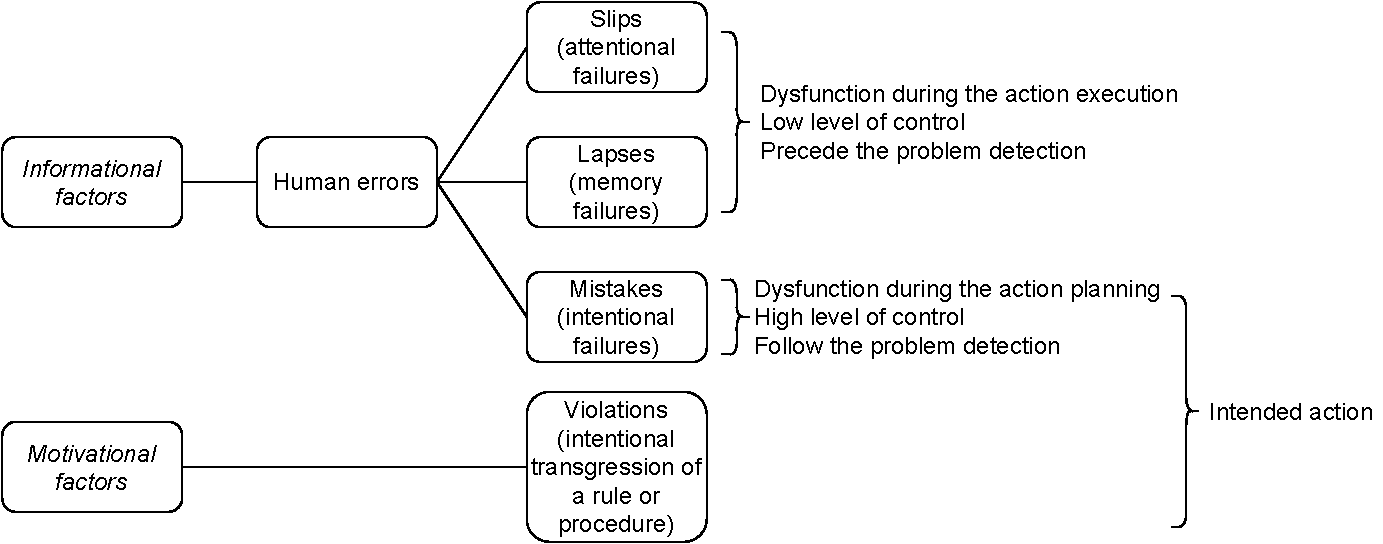
\includegraphics[width=\linewidth]{figures/chapter1/reason-errors.pdf}
 	\caption{Summary and simplification of the failure classification (Generic Error-Modelling System (GEMS) and violations) developed by Reason~\cite{reason_1990_human}. (Illustration by Kathleen Belhassein)}
 	\label{chap1:fig:err}
 \end{figure}


\subsection{Repair strategies}
In psychology or philosophy, there are not a lot of work on what happens once an error has been made during a joint action. Conversation Analysis investigated repair, which is a way to correct a misunderstanding or an error during an interaction or an action. The ability to engage in repair is essential in interactions. Indeed, errors and misunderstandings are likely to arise and people should find ways to correct them. Generally, they are classified in four categories in CA \cite{schegloff_1977_preference,wooffitt_2008_conversation}:
\begin{bulletList}
	\item Self-initiated self-repair: Repair is both initiated and carried out by the responsible of the trouble
	\item Other-initiated self-repair: The responsible of the trouble takes care of the repair himself but the trouble have been pointed out by the other
	\item Self-initiated other-repair: The responsible of the trouble signals that a repair is needed and get the other one to repair (\eg he forgot a name and asks for help to remember)
	\item Other-initiated other-repair: The one not responsible of the trouble initiates and carries out the repair. This is closest to what is conventionally understood as ``correction''.
\end{bulletList}
\end{comment}

\ifdefined\included
\else
\bibliographystyle{acm}
\bibliography{These}
\end{document}
\fi
